\documentclass[]{article}
\usepackage{lmodern}
\usepackage{amssymb,amsmath}
\usepackage{ifxetex,ifluatex}
\usepackage{fixltx2e} % provides \textsubscript
\ifnum 0\ifxetex 1\fi\ifluatex 1\fi=0 % if pdftex
  \usepackage[T1]{fontenc}
  \usepackage[utf8]{inputenc}
\else % if luatex or xelatex
  \ifxetex
    \usepackage{mathspec}
  \else
    \usepackage{fontspec}
  \fi
  \defaultfontfeatures{Ligatures=TeX,Scale=MatchLowercase}
\fi
% use upquote if available, for straight quotes in verbatim environments
\IfFileExists{upquote.sty}{\usepackage{upquote}}{}
% use microtype if available
\IfFileExists{microtype.sty}{%
\usepackage{microtype}
\UseMicrotypeSet[protrusion]{basicmath} % disable protrusion for tt fonts
}{}
\usepackage[margin=1in]{geometry}
\usepackage{hyperref}
\hypersetup{unicode=true,
            pdftitle={Red Wine Dataset Analysis},
            pdfauthor={Patrick Flynn},
            pdfborder={0 0 0},
            breaklinks=true}
\urlstyle{same}  % don't use monospace font for urls
\usepackage{color}
\usepackage{fancyvrb}
\newcommand{\VerbBar}{|}
\newcommand{\VERB}{\Verb[commandchars=\\\{\}]}
\DefineVerbatimEnvironment{Highlighting}{Verbatim}{commandchars=\\\{\}}
% Add ',fontsize=\small' for more characters per line
\usepackage{framed}
\definecolor{shadecolor}{RGB}{248,248,248}
\newenvironment{Shaded}{\begin{snugshade}}{\end{snugshade}}
\newcommand{\AlertTok}[1]{\textcolor[rgb]{0.94,0.16,0.16}{#1}}
\newcommand{\AnnotationTok}[1]{\textcolor[rgb]{0.56,0.35,0.01}{\textbf{\textit{#1}}}}
\newcommand{\AttributeTok}[1]{\textcolor[rgb]{0.77,0.63,0.00}{#1}}
\newcommand{\BaseNTok}[1]{\textcolor[rgb]{0.00,0.00,0.81}{#1}}
\newcommand{\BuiltInTok}[1]{#1}
\newcommand{\CharTok}[1]{\textcolor[rgb]{0.31,0.60,0.02}{#1}}
\newcommand{\CommentTok}[1]{\textcolor[rgb]{0.56,0.35,0.01}{\textit{#1}}}
\newcommand{\CommentVarTok}[1]{\textcolor[rgb]{0.56,0.35,0.01}{\textbf{\textit{#1}}}}
\newcommand{\ConstantTok}[1]{\textcolor[rgb]{0.00,0.00,0.00}{#1}}
\newcommand{\ControlFlowTok}[1]{\textcolor[rgb]{0.13,0.29,0.53}{\textbf{#1}}}
\newcommand{\DataTypeTok}[1]{\textcolor[rgb]{0.13,0.29,0.53}{#1}}
\newcommand{\DecValTok}[1]{\textcolor[rgb]{0.00,0.00,0.81}{#1}}
\newcommand{\DocumentationTok}[1]{\textcolor[rgb]{0.56,0.35,0.01}{\textbf{\textit{#1}}}}
\newcommand{\ErrorTok}[1]{\textcolor[rgb]{0.64,0.00,0.00}{\textbf{#1}}}
\newcommand{\ExtensionTok}[1]{#1}
\newcommand{\FloatTok}[1]{\textcolor[rgb]{0.00,0.00,0.81}{#1}}
\newcommand{\FunctionTok}[1]{\textcolor[rgb]{0.00,0.00,0.00}{#1}}
\newcommand{\ImportTok}[1]{#1}
\newcommand{\InformationTok}[1]{\textcolor[rgb]{0.56,0.35,0.01}{\textbf{\textit{#1}}}}
\newcommand{\KeywordTok}[1]{\textcolor[rgb]{0.13,0.29,0.53}{\textbf{#1}}}
\newcommand{\NormalTok}[1]{#1}
\newcommand{\OperatorTok}[1]{\textcolor[rgb]{0.81,0.36,0.00}{\textbf{#1}}}
\newcommand{\OtherTok}[1]{\textcolor[rgb]{0.56,0.35,0.01}{#1}}
\newcommand{\PreprocessorTok}[1]{\textcolor[rgb]{0.56,0.35,0.01}{\textit{#1}}}
\newcommand{\RegionMarkerTok}[1]{#1}
\newcommand{\SpecialCharTok}[1]{\textcolor[rgb]{0.00,0.00,0.00}{#1}}
\newcommand{\SpecialStringTok}[1]{\textcolor[rgb]{0.31,0.60,0.02}{#1}}
\newcommand{\StringTok}[1]{\textcolor[rgb]{0.31,0.60,0.02}{#1}}
\newcommand{\VariableTok}[1]{\textcolor[rgb]{0.00,0.00,0.00}{#1}}
\newcommand{\VerbatimStringTok}[1]{\textcolor[rgb]{0.31,0.60,0.02}{#1}}
\newcommand{\WarningTok}[1]{\textcolor[rgb]{0.56,0.35,0.01}{\textbf{\textit{#1}}}}
\usepackage{graphicx,grffile}
\makeatletter
\def\maxwidth{\ifdim\Gin@nat@width>\linewidth\linewidth\else\Gin@nat@width\fi}
\def\maxheight{\ifdim\Gin@nat@height>\textheight\textheight\else\Gin@nat@height\fi}
\makeatother
% Scale images if necessary, so that they will not overflow the page
% margins by default, and it is still possible to overwrite the defaults
% using explicit options in \includegraphics[width, height, ...]{}
\setkeys{Gin}{width=\maxwidth,height=\maxheight,keepaspectratio}
\IfFileExists{parskip.sty}{%
\usepackage{parskip}
}{% else
\setlength{\parindent}{0pt}
\setlength{\parskip}{6pt plus 2pt minus 1pt}
}
\setlength{\emergencystretch}{3em}  % prevent overfull lines
\providecommand{\tightlist}{%
  \setlength{\itemsep}{0pt}\setlength{\parskip}{0pt}}
\setcounter{secnumdepth}{0}
% Redefines (sub)paragraphs to behave more like sections
\ifx\paragraph\undefined\else
\let\oldparagraph\paragraph
\renewcommand{\paragraph}[1]{\oldparagraph{#1}\mbox{}}
\fi
\ifx\subparagraph\undefined\else
\let\oldsubparagraph\subparagraph
\renewcommand{\subparagraph}[1]{\oldsubparagraph{#1}\mbox{}}
\fi

%%% Use protect on footnotes to avoid problems with footnotes in titles
\let\rmarkdownfootnote\footnote%
\def\footnote{\protect\rmarkdownfootnote}

%%% Change title format to be more compact
\usepackage{titling}

% Create subtitle command for use in maketitle
\providecommand{\subtitle}[1]{
  \posttitle{
    \begin{center}\large#1\end{center}
    }
}

\setlength{\droptitle}{-2em}

  \title{Red Wine Dataset Analysis}
    \pretitle{\vspace{\droptitle}\centering\huge}
  \posttitle{\par}
    \author{Patrick Flynn}
    \preauthor{\centering\large\emph}
  \postauthor{\par}
      \predate{\centering\large\emph}
  \postdate{\par}
    \date{6/3/2019}


\begin{document}
\maketitle

\hypertarget{introduction}{%
\subsection{Introduction}\label{introduction}}

The dataset used in this analysis is the red wine dataset described in
Cortez et al., 2009. The red wine dataset contains 1599 observations of
red wine samples. For each sample, chemical analysis was completed and
the wine was rated by wine experts. The wine experts rated a particular
wine on a 1-10 scale represented in this dataset by the
\emph{``quality''} variable.

\hypertarget{variables-in-dataset-described-in-data}{%
\subsubsection{Variables in Dataset (Described in
data)}\label{variables-in-dataset-described-in-data}}

\textbf{Input variables (based on physicochemical tests):}

\begin{enumerate}
\def\labelenumi{\arabic{enumi}.}
\tightlist
\item
  fixed acidity (tartaric acid - g / dm\^{}3)

  \begin{itemize}
  \tightlist
  \item
    most acids involved with wine or fixed or nonvolatile (do not
    evaporate readily)
  \end{itemize}
\item
  volatile acidity (acetic acid - g / dm\^{}3)

  \begin{itemize}
  \tightlist
  \item
    the amount of acetic acid in wine, which at too high of levels can
    lead to an unpleasant, vinegar taste
  \end{itemize}
\item
  citric acid (g / dm\^{}3)

  \begin{itemize}
  \tightlist
  \item
    found in small quantities, citric acid can add `freshness' and
    flavor to wines
  \end{itemize}
\item
  residual sugar (g / dm\^{}3)

  \begin{itemize}
  \tightlist
  \item
    the amount of sugar remaining after fermentation stops, it's rare to
    find wines with less than 1 gram/liter and wines with greater than
    45 grams/liter are considered sweet
  \end{itemize}
\item
  chlorides (sodium chloride - g / dm\^{}3

  \begin{itemize}
  \tightlist
  \item
    the amount of salt in the wine
  \end{itemize}
\item
  free sulfur dioxide (mg / dm\^{}3)

  \begin{itemize}
  \tightlist
  \item
    the free form of SO2 exists in equilibrium between molecular SO2 (as
    a dissolved gas) and bisulfite ion; it prevents microbial growth and
    the oxidation of wine
  \end{itemize}
\item
  total sulfur dioxide (mg / dm\^{}3)

  \begin{itemize}
  \tightlist
  \item
    total sulfur dioxide: amount of free and bound forms of S02; in low
    concentrations, SO2 is mostly undetectable in wine, but at free SO2
    concentrations over 50 ppm, SO2 becomes evident in the nose and
    taste of wine
  \end{itemize}
\item
  density (g / cm\^{}3)

  \begin{itemize}
  \tightlist
  \item
    the density of water is close to that of water depending on the
    percent alcohol and sugar content
  \end{itemize}
\item
  pH

  \begin{itemize}
  \tightlist
  \item
    describes how acidic or basic a wine is on a scale from 0 (very
    acidic) to 14 (very basic); most wines are between 3-4 on the pH
    scale
  \end{itemize}
\item
  sulphates (potassium sulphate - g / dm3)

  \begin{itemize}
  \tightlist
  \item
    a wine additive which can contribute to sulfur dioxide gas (S02)
    levels, wich acts as an antimicrobial and antioxidant
  \end{itemize}
\item
  alcohol (\% by volume)

  \begin{itemize}
  \tightlist
  \item
    the percent alcohol content of the wine
  \end{itemize}
\end{enumerate}

\textbf{Output variable (based on sensory data):}

\begin{enumerate}
\def\labelenumi{\arabic{enumi}.}
\setcounter{enumi}{11}
\tightlist
\item
  quality (score between 0 and 10)
\end{enumerate}

\begin{quote}
\textbf{Data Source:} P. Cortez, A. Cerdeira, F. Almeida, T. Matos and
J. Reis. Modeling wine preferences by data mining from physicochemical
properties. In Decision Support Systems, Elsevier, 47(4):547-553. ISSN:
0167-9236.
\end{quote}

Wine Dataset Summary Statistics:

\begin{verbatim}
##        X          fixed.acidity   volatile.acidity  citric.acid   
##  Min.   :   1.0   Min.   : 4.60   Min.   :0.1200   Min.   :0.000  
##  1st Qu.: 400.5   1st Qu.: 7.10   1st Qu.:0.3900   1st Qu.:0.090  
##  Median : 800.0   Median : 7.90   Median :0.5200   Median :0.260  
##  Mean   : 800.0   Mean   : 8.32   Mean   :0.5278   Mean   :0.271  
##  3rd Qu.:1199.5   3rd Qu.: 9.20   3rd Qu.:0.6400   3rd Qu.:0.420  
##  Max.   :1599.0   Max.   :15.90   Max.   :1.5800   Max.   :1.000  
##  residual.sugar     chlorides       free.sulfur.dioxide
##  Min.   : 0.900   Min.   :0.01200   Min.   : 1.00      
##  1st Qu.: 1.900   1st Qu.:0.07000   1st Qu.: 7.00      
##  Median : 2.200   Median :0.07900   Median :14.00      
##  Mean   : 2.539   Mean   :0.08747   Mean   :15.87      
##  3rd Qu.: 2.600   3rd Qu.:0.09000   3rd Qu.:21.00      
##  Max.   :15.500   Max.   :0.61100   Max.   :72.00      
##  total.sulfur.dioxide    density             pH          sulphates     
##  Min.   :  6.00       Min.   :0.9901   Min.   :2.740   Min.   :0.3300  
##  1st Qu.: 22.00       1st Qu.:0.9956   1st Qu.:3.210   1st Qu.:0.5500  
##  Median : 38.00       Median :0.9968   Median :3.310   Median :0.6200  
##  Mean   : 46.47       Mean   :0.9967   Mean   :3.311   Mean   :0.6581  
##  3rd Qu.: 62.00       3rd Qu.:0.9978   3rd Qu.:3.400   3rd Qu.:0.7300  
##  Max.   :289.00       Max.   :1.0037   Max.   :4.010   Max.   :2.0000  
##     alcohol         quality     
##  Min.   : 8.40   Min.   :3.000  
##  1st Qu.: 9.50   1st Qu.:5.000  
##  Median :10.20   Median :6.000  
##  Mean   :10.42   Mean   :5.636  
##  3rd Qu.:11.10   3rd Qu.:6.000  
##  Max.   :14.90   Max.   :8.000
\end{verbatim}

\begin{verbatim}
## `stat_bin()` using `bins = 30`. Pick better value with `binwidth`.
\end{verbatim}

\includegraphics{RedWineAnalysisPatrickFlynn_files/figure-latex/unnamed-chunk-1-1.pdf}

\begin{verbatim}
## Warning: Ignoring unknown parameters: fun.x
\end{verbatim}

\begin{verbatim}
## No summary function supplied, defaulting to `mean_se()
\end{verbatim}

\includegraphics{RedWineAnalysisPatrickFlynn_files/figure-latex/unnamed-chunk-1-2.pdf}

\hypertarget{univariate-plots-section}{%
\section{Univariate Plots Section}\label{univariate-plots-section}}

Various single measures of the wine will be expalained in this portion
of the analysis. Based on findings, analysis will be done on the
relationship between various sets of measures.

\hypertarget{wine-quality}{%
\subsection{Wine Quality}\label{wine-quality}}

How well were the wines rated?

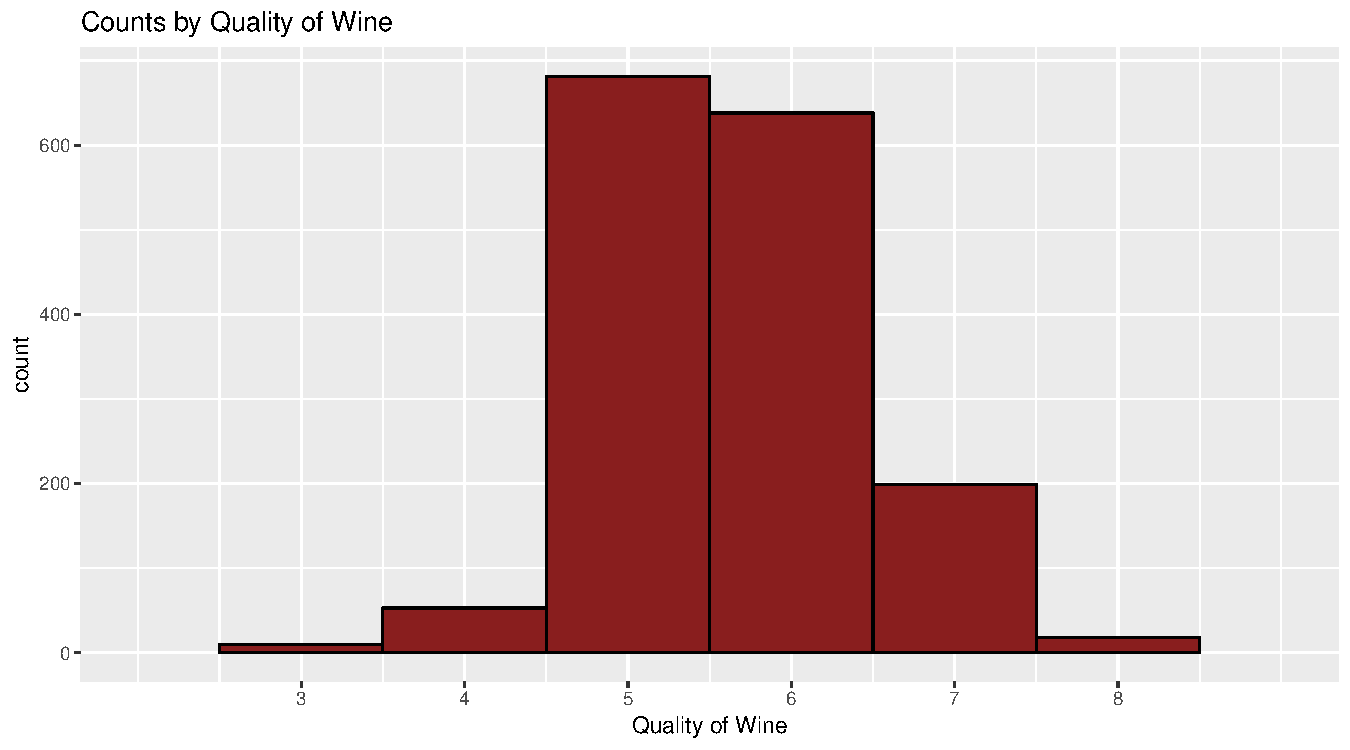
\includegraphics{RedWineAnalysisPatrickFlynn_files/figure-latex/unnamed-chunk-2-1.pdf}

The above chart describes the distribution of quality ratings amongst
the wine samples. The wines are very heavily distributed in the 5 and 6
quality ratings. On the high quality end, There are no wines that scored
a 9 or 10. Likewise, no wines scored a 1 or 2. These wines were mediocre
based on the qualities rated by the wine experts.

The summary statistics are as follows for the quality ratings of the
wine:

\begin{verbatim}
##    Min. 1st Qu.  Median    Mean 3rd Qu.    Max. 
##   3.000   5.000   6.000   5.636   6.000   8.000
\end{verbatim}

\hypertarget{wine-alcohol-content}{%
\subsection{Wine Alcohol Content}\label{wine-alcohol-content}}

How high/low is the alcohol content?

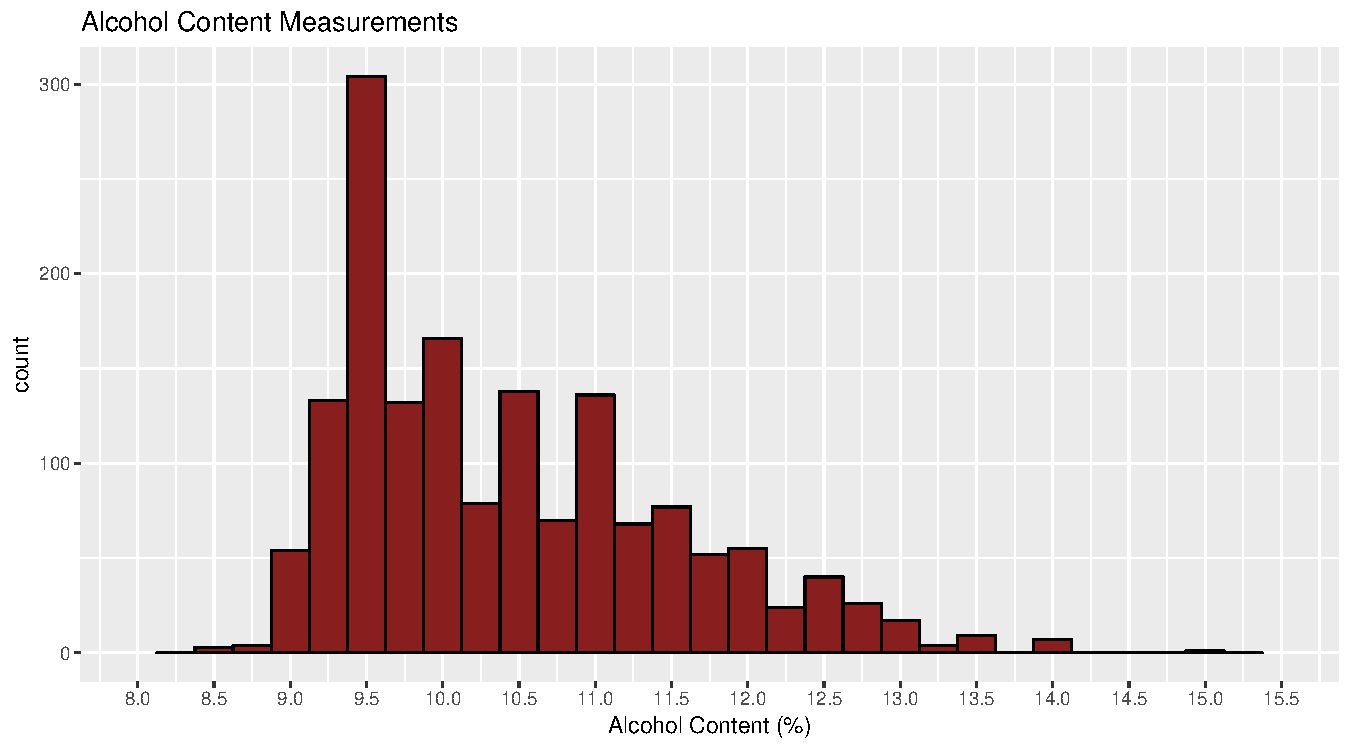
\includegraphics{RedWineAnalysisPatrickFlynn_files/figure-latex/unnamed-chunk-4-1.pdf}

The majority of the wine samples in our data fall between 8\% and 11\%
alcohol content by volume. A large number of the wine samples are
concentrated around 9.5\% alcohol by volume. Only a small amount of the
wine samples are above 12\%. According to Alchol.Org, most red wines are
typically between 12-15\%
\href{https://www.alcohol.org/statistics-information/abv/}{Source}.
Perhaps this is why our quality was lower? We will explore this
relationship further in our analysis.

The summary statistics are as follows for the alcohol content of the
wine:

\begin{verbatim}
##    Min. 1st Qu.  Median    Mean 3rd Qu.    Max. 
##    8.40    9.50   10.20   10.42   11.10   14.90
\end{verbatim}

This is an R Markdown document. Markdown is a simple formatting syntax
for authoring HTML, PDF, and MS Word documents. For more details on
using R Markdown see \url{http://rmarkdown.rstudio.com}.

When you click the \textbf{Knit} button a document will be generated
that includes both content as well as the output of any embedded R code
chunks within the document. You can embed an R code chunk like this:

\begin{Shaded}
\begin{Highlighting}[]
\KeywordTok{summary}\NormalTok{(cars)}
\end{Highlighting}
\end{Shaded}

\begin{verbatim}
##      speed           dist       
##  Min.   : 4.0   Min.   :  2.00  
##  1st Qu.:12.0   1st Qu.: 26.00  
##  Median :15.0   Median : 36.00  
##  Mean   :15.4   Mean   : 42.98  
##  3rd Qu.:19.0   3rd Qu.: 56.00  
##  Max.   :25.0   Max.   :120.00
\end{verbatim}

\begin{Shaded}
\begin{Highlighting}[]
\KeywordTok{print}\NormalTok{(}\StringTok{"hello!"}\NormalTok{)}
\end{Highlighting}
\end{Shaded}

\begin{verbatim}
## [1] "hello!"
\end{verbatim}

\hypertarget{including-plots}{%
\subsection{Including Plots}\label{including-plots}}

You can also embed plots, for example:

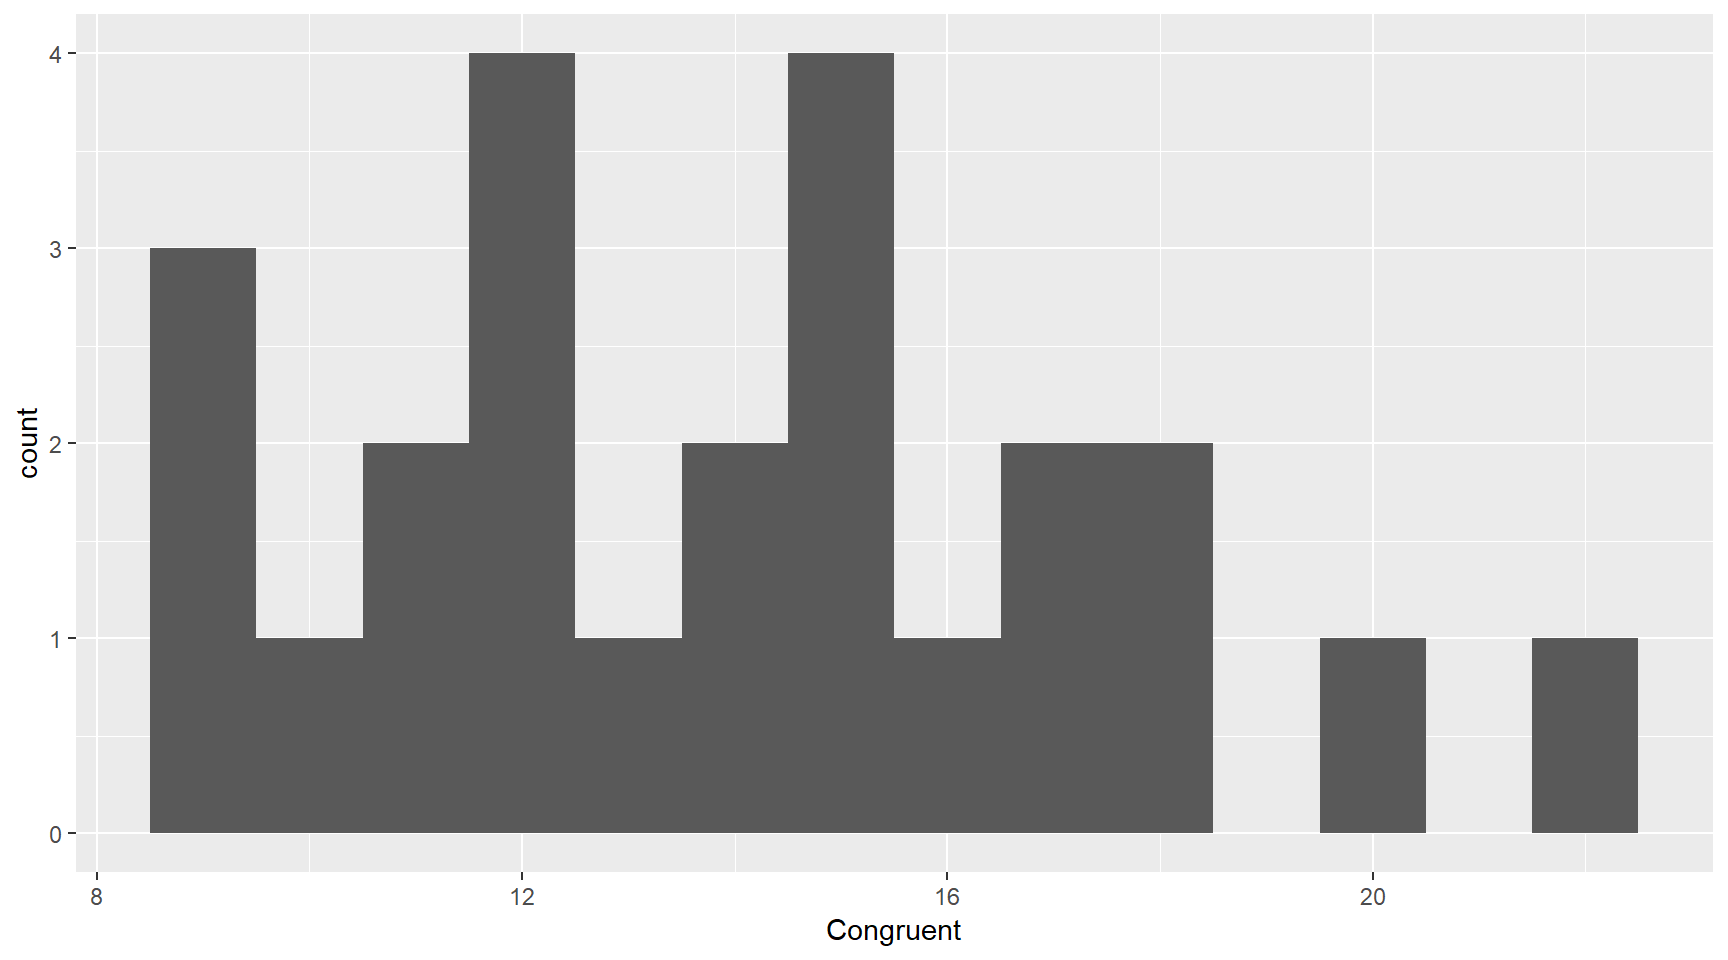
\includegraphics{RedWineAnalysisPatrickFlynn_files/figure-latex/pressure-1.pdf}

Note that the \texttt{echo\ =\ FALSE} parameter was added to the code
chunk to prevent printing of the R code that generated the plot.

\hypertarget{title-by-your_name_here}{%
\section{TITLE by YOUR\_NAME\_HERE}\label{title-by-your_name_here}}

\begin{quote}
\textbf{Tip}: You will see quoted sections like this throughout the
template to help you construct your report. Make sure that you remove
these notes before you finish and submit your project!
\end{quote}

\begin{quote}
\textbf{Tip}: One of the requirements of this project is that your code
follows good formatting techniques, including limiting your lines to 80
characters or less. If you're using RStudio, go into Preferences
\textgreater{} Code \textgreater{} Display to set up a margin line to
help you keep track of this guideline!
\end{quote}

\begin{quote}
\textbf{Tip}: Before you create any plots, it is a good idea to provide
a short introduction into the dataset that you are planning to explore.
Replace this quoted text with that general information!
\end{quote}

\hypertarget{univariate-plots-section-1}{%
\section{Univariate Plots Section}\label{univariate-plots-section-1}}

\begin{quote}
\textbf{Tip}: In this section, you should perform some preliminary
exploration of your dataset. Run some summaries of the data and create
univariate plots to understand the structure of the individual variables
in your dataset. Don't forget to add a comment after each plot or
closely-related group of plots! There should be multiple code chunks and
text sections; the first one below is just to help you get started.
\end{quote}

\begin{quote}
\textbf{Tip}: Make sure that you leave a blank line between the start /
end of each code block and the end / start of your Markdown text so that
it is formatted nicely in the knitted text. Note as well that text on
consecutive lines is treated as a single space. Make sure you have a
blank line between your paragraphs so that they too are formatted for
easy readability.
\end{quote}

\hypertarget{univariate-analysis}{%
\section{Univariate Analysis}\label{univariate-analysis}}

\begin{quote}
\textbf{Tip}: Now that you've completed your univariate explorations,
it's time to reflect on and summarize what you've found. Use the
questions below to help you gather your observations and add your own if
you have other thoughts!
\end{quote}

\hypertarget{what-is-the-structure-of-your-dataset}{%
\subsubsection{What is the structure of your
dataset?}\label{what-is-the-structure-of-your-dataset}}

\hypertarget{what-isare-the-main-features-of-interest-in-your-dataset}{%
\subsubsection{What is/are the main feature(s) of interest in your
dataset?}\label{what-isare-the-main-features-of-interest-in-your-dataset}}

\hypertarget{what-other-features-in-the-dataset-do-you-think-will-help-support-your}{%
\subsubsection{\texorpdfstring{What other features in the dataset do you
think will help support your\\
}{What other features in the dataset do you think will help support your }}\label{what-other-features-in-the-dataset-do-you-think-will-help-support-your}}

investigation into your feature(s) of interest?

\hypertarget{did-you-create-any-new-variables-from-existing-variables-in-the-dataset}{%
\subsubsection{Did you create any new variables from existing variables
in the
dataset?}\label{did-you-create-any-new-variables-from-existing-variables-in-the-dataset}}

\hypertarget{of-the-features-you-investigated-were-there-any-unusual-distributions}{%
\subsubsection{\texorpdfstring{Of the features you investigated, were
there any unusual distributions?\\
}{Of the features you investigated, were there any unusual distributions? }}\label{of-the-features-you-investigated-were-there-any-unusual-distributions}}

Did you perform any operations on the data to tidy, adjust, or change
the form\\
of the data? If so, why did you do this?

\hypertarget{bivariate-plots-section}{%
\section{Bivariate Plots Section}\label{bivariate-plots-section}}

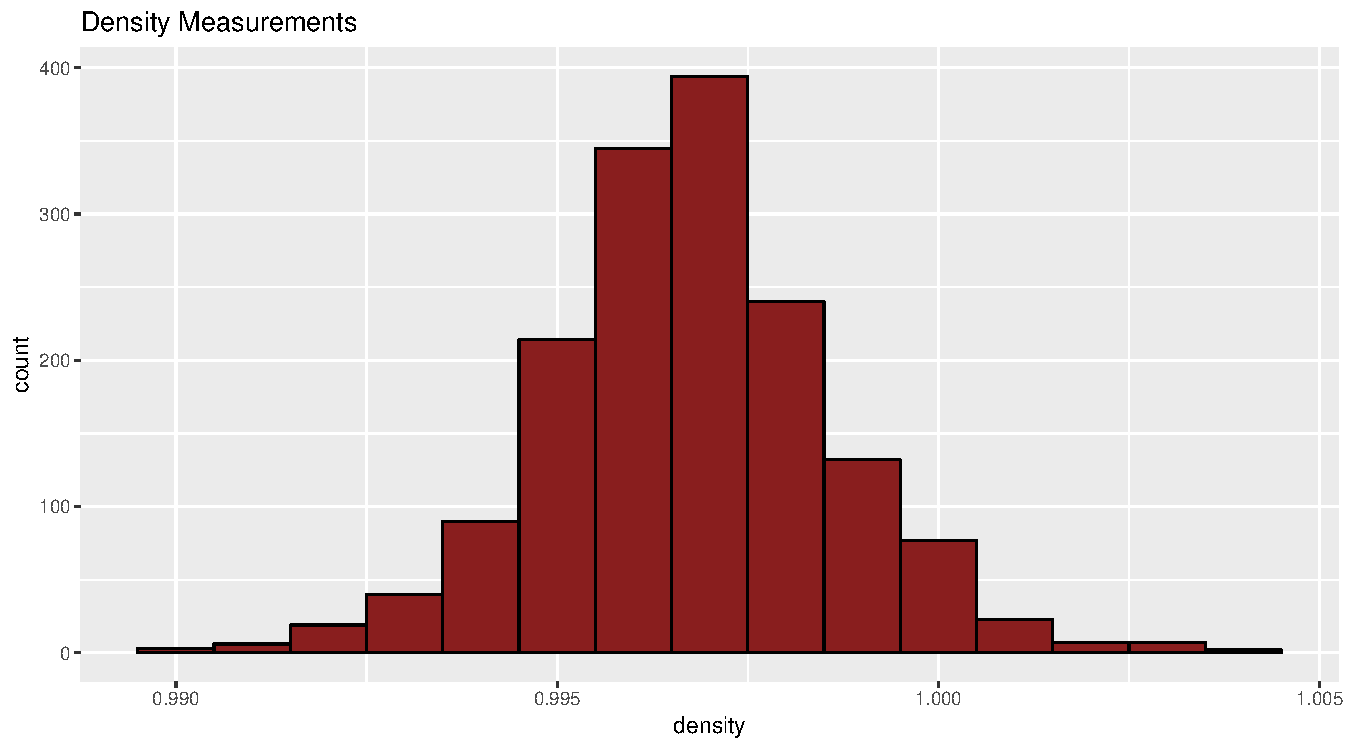
\includegraphics{RedWineAnalysisPatrickFlynn_files/figure-latex/unnamed-chunk-6-1.pdf}

\begin{quote}
\textbf{Tip}: Based on what you saw in the univariate plots, what
relationships between variables might be interesting to look at in this
section? Don't limit yourself to relationships between a main output
feature and one of the supporting variables. Try to look at
relationships between supporting variables as well.
\end{quote}

\hypertarget{bivariate-analysis}{%
\section{Bivariate Analysis}\label{bivariate-analysis}}

\begin{quote}
\textbf{Tip}: As before, summarize what you found in your bivariate
explorations here. Use the questions below to guide your discussion.
\end{quote}

\hypertarget{talk-about-some-of-the-relationships-you-observed-in-this-part-of-the}{%
\subsubsection{\texorpdfstring{Talk about some of the relationships you
observed in this part of the\\
}{Talk about some of the relationships you observed in this part of the }}\label{talk-about-some-of-the-relationships-you-observed-in-this-part-of-the}}

investigation. How did the feature(s) of interest vary with other
features in\\
the dataset?

\hypertarget{did-you-observe-any-interesting-relationships-between-the-other-features}{%
\subsubsection{\texorpdfstring{Did you observe any interesting
relationships between the other features\\
}{Did you observe any interesting relationships between the other features }}\label{did-you-observe-any-interesting-relationships-between-the-other-features}}

(not the main feature(s) of interest)?

\hypertarget{what-was-the-strongest-relationship-you-found}{%
\subsubsection{What was the strongest relationship you
found?}\label{what-was-the-strongest-relationship-you-found}}

\hypertarget{multivariate-plots-section}{%
\section{Multivariate Plots Section}\label{multivariate-plots-section}}

\begin{quote}
\textbf{Tip}: Now it's time to put everything together. Based on what
you found in the bivariate plots section, create a few multivariate
plots to investigate more complex interactions between variables. Make
sure that the plots that you create here are justified by the plots you
explored in the previous section. If you plan on creating any
mathematical models, this is the section where you will do that.
\end{quote}

\hypertarget{multivariate-analysis}{%
\section{Multivariate Analysis}\label{multivariate-analysis}}

\hypertarget{talk-about-some-of-the-relationships-you-observed-in-this-part-of-the-1}{%
\subsubsection{\texorpdfstring{Talk about some of the relationships you
observed in this part of the\\
}{Talk about some of the relationships you observed in this part of the }}\label{talk-about-some-of-the-relationships-you-observed-in-this-part-of-the-1}}

investigation. Were there features that strengthened each other in terms
of\\
looking at your feature(s) of interest?

\hypertarget{were-there-any-interesting-or-surprising-interactions-between-features}{%
\subsubsection{Were there any interesting or surprising interactions
between
features?}\label{were-there-any-interesting-or-surprising-interactions-between-features}}

\hypertarget{optional-did-you-create-any-models-with-your-dataset-discuss-the}{%
\subsubsection{\texorpdfstring{OPTIONAL: Did you create any models with
your dataset? Discuss the\\
}{OPTIONAL: Did you create any models with your dataset? Discuss the }}\label{optional-did-you-create-any-models-with-your-dataset-discuss-the}}

strengths and limitations of your model.

\begin{center}\rule{0.5\linewidth}{\linethickness}\end{center}

\hypertarget{final-plots-and-summary}{%
\section{Final Plots and Summary}\label{final-plots-and-summary}}

\begin{quote}
\textbf{Tip}: You've done a lot of exploration and have built up an
understanding of the structure of and relationships between the
variables in your dataset. Here, you will select three plots from all of
your previous exploration to present here as a summary of some of your
most interesting findings. Make sure that you have refined your selected
plots for good titling, axis labels (with units), and good aesthetic
choices (e.g.~color, transparency). After each plot, make sure you
justify why you chose each plot by describing what it shows.
\end{quote}

\hypertarget{plot-one}{%
\subsubsection{Plot One}\label{plot-one}}

\hypertarget{description-one}{%
\subsubsection{Description One}\label{description-one}}

\hypertarget{plot-two}{%
\subsubsection{Plot Two}\label{plot-two}}

\hypertarget{description-two}{%
\subsubsection{Description Two}\label{description-two}}

\hypertarget{plot-three}{%
\subsubsection{Plot Three}\label{plot-three}}

\hypertarget{description-three}{%
\subsubsection{Description Three}\label{description-three}}

\begin{center}\rule{0.5\linewidth}{\linethickness}\end{center}

\hypertarget{reflection}{%
\section{Reflection}\label{reflection}}

\begin{quote}
\textbf{Tip}: Here's the final step! Reflect on the exploration you
performed and the insights you found. What were some of the struggles
that you went through? What went well? What was surprising? Make sure
you include an insight into future work that could be done with the
dataset.
\end{quote}

\begin{quote}
\textbf{Tip}: Don't forget to remove this, and the other \textbf{Tip}
sections before saving your final work and knitting the final report!
\end{quote}


\end{document}
